\documentclass{ximera}

\outcome{Put together everything learned in this class so far to determine how the graph of a function looks without using a graphing calculator.}

\title{graphing functions}

\begin{document}

\begin{abstract}
  We can now use calculus to graph functions by hand
\end{abstract}

\maketitle


\begin{image}
  \begin{tikzpicture}
    \colorlet{textColor}{black}
    \colorlet{penColor}{blue!50!black}
	\begin{axis}[
            domain=-5:5,
            ymax=8,
            ymin=-8,
            width=6in,
            %samples=100,
            axis lines =middle, xlabel=$x$, ylabel=$y$,
            every axis y label/.style={at=(current axis.above origin),anchor=south},
            every axis x label/.style={at=(current axis.right of origin),anchor=west}
          ]
      
          \addplot [thick, penColor, smooth,domain=(-5:-1.1)] {x/(x^2-1)};
          \addplot [thick, penColor, smooth,domain=(-0.9:0.9)] {x/(x^2-1)};
          \addplot [thick, penColor, smooth,domain=(1.1:5)] {x/(x^2-1)};
          \addplot [dashed, textColor, smooth] plot coordinates {(1,8) (1,-8)};
          \addplot [dashed, textColor, smooth] plot coordinates {(-1,8) (-1,-8)};
        \end{axis}
\end{tikzpicture}
\end{image}

This prefecture is one long extended exercise.  We will learn everything we can about the function $f(x) = \frac{x}{x^2-1}$, and use this information to graph $f$.
\textbf{Do not} use a graphing calculator to help you during this activity.  It will rob you of the whole experience.

\begin{question}

\textbf{Domain}

\begin{solution}
What is the domain of $f$?
 
    \begin{multipleChoice}
      \choice[correct]{$\mathbb{R}-\{-1,1\}$}
      \choice{$(1,\infty)$}
      \choice{$(-\infty,1)$}
      \choice{$(-1,1)$}
    \end{multipleChoice}
    
\end{solution}    

\textbf{Symmetry}

\begin{solution}
   What sort of symmetry does $f$ have?
   
    \begin{multipleChoice}
      \choice[correct]{odd}
      \choice{even}
      \choice{symmetry about the lines $x=1$ and $x=-1$ }
      \choice{symmetry about the points $(1,0)$ and $(-1,0)$}
    \end{multipleChoice}

\end{solution}    

    Right!  So we only have to graph $f$ on $[0,\infty)$, and use symmetry to graph it on the other half of its domain.
    
 \textbf{Find First and Second Derivative}
 
 \begin{solution}
 	$f'(x)=$\answer{-2*x^2/(x^2 - 1)^2 + 1/(x^2 - 1)}
 \end{solution}
 
 \begin{solution}
 	$f''(x)=$\answer{8*x^3/(x^2 - 1)^3 - 6*x/(x^2 - 1)^2}
 \end{solution}
 
 \textbf{Find the Critical Points and Possible Inflection Points}
 
 \begin{solution}
	Now find all of the points where $f'(x)=0$ or does not exist (critical points), and where $f''(x)=0$ or does not exist (possible inflection points).
	
	Which of the following sets is the set of all critical points and possible inflection points of $f$ on the interval $[0,\infty)$?
	
	 \begin{multipleChoice}
     \choice[correct]{$\{1\}$}
      \choice{$\{1,2\}$}
      \choice{$\{8,6\}$ }
      \choice{There are no critical points or possible inflection points}
    \end{multipleChoice}

 \end{solution}
 
 \textbf{Identify Increasing/Decreasing Behavior and Convaity}
 
 \begin{solution}
 On the interval $(0,1)$ $f$ is
 
 \begin{multipleChoice}
     \choice[correct]{Decreasing and concave down}
      \choice{Decreasing and concave up}
      \choice{Increasing and concave down}
      \choice{Increasing and concave up}
    \end{multipleChoice}
    
  On the interval $(1,\infty)$ $f$ is
 
  \begin{multipleChoice}
     \choice[correct]{Decreasing and concave up}
      \choice{Decreasing and concave down}
      \choice{Increasing and concave down}
      \choice{Increasing and concave up}
    \end{multipleChoice}
    \end{solution}
    
 \textbf{Identify extreme values and inflection points}
 
 Ordinarily, this would be a major step, but in our case, the only critical point is $x=1$, and $f$ is undefined there, so we skip this step.
 
 \textbf{Locate vertical/horizontal asymptotes and determine end behavior}
 
 \begin{solution}
 Which of the following are true?
 
 \begin{multipleChoice}
     \choice[correct]{$\lim_{x \to 1^-} f(x) = -\infty$, $\lim_{x \to 1^+} f(x) = \infty$, and $\lim_{x \to \infty} f(x) = 0$}
      \choice{$\lim_{x \to 1^-} f(x) = -\infty$, $\lim_{x \to 1^+} f(x) = \infty$, and $\lim_{x \to \infty} f(x) = \infty$}
      \choice{$\lim_{x \to 1^-} f(x) = \infty$, $\lim_{x \to 1^+} f(x) = \infty$, and $\lim_{x \to \infty} f(x) = 0$}
      \choice{$\lim_{x \to 1^-} f(x) = \infty$, $\lim_{x \to 1^+} f(x) = -\infty$, and $\lim_{x \to \infty} f(x) = -\infty$}
    \end{multipleChoice}
    \end{solution}
  \textbf{Find the Intercepts}
  
  In this case, we can see that the only zero of $f$ occurs when $x=0$.  So the function passes through the origin, and this is the only $x$ or $y$ intercept.
  
  \textbf{Choose an Appropriate Graphing Window and Make a Graph}
  
  Try to graph the function now, using all of the information you have gathered above.  
  
  
  \begin{solution}
  
  Do you solemnly swear that you tried to graph it on your own?  We will reveal the graph after you say "yes", so that you can compare your work with the correct answer.
  
  	\begin{multipleChoice}
     \choice[correct]{yes}
      \choice{no}
    \end{multipleChoice}

  \end{solution}
  
       
\begin{image}
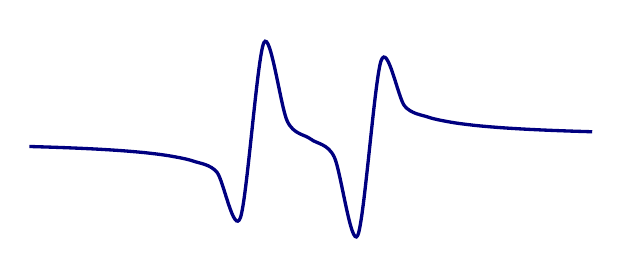
\begin{tikzpicture}
  \colorlet{textColor}{black}
  \colorlet{penColor}{blue!50!black}
	\begin{axis}[
            domain=-5:5,
            ymax=8,
            width=4in,
            ymin=-8,
            axis lines=none,
          ]
          \addplot [very thick, penColor, smooth, domain=(-5:5)] {x/(x^2-1)};
        \end{axis}
\end{tikzpicture}
\end{image}

\begin{image}
  \begin{tikzpicture}
    \colorlet{textColor}{black}
    \colorlet{penColor}{blue!50!black}
	\begin{axis}[
            domain=-5:5,
            ymax=8,
            ymin=-8,
            width=6in,
            %samples=100,
            axis lines =middle, xlabel=$x$, ylabel=$y$,
            every axis y label/.style={at=(current axis.above origin),anchor=south},
            every axis x label/.style={at=(current axis.right of origin),anchor=west}
          ]
      
          \addplot [thick, penColor, smooth,domain=(-5:-1.1)] {x/(x^2-1)};
          \addplot [thick, penColor, smooth,domain=(-0.9:0.9)] {x/(x^2-1)};
          \addplot [thick, penColor, smooth,domain=(1.1:5)] {x/(x^2-1)};
          \addplot [dashed, textColor, smooth] plot coordinates {(1,8) (1,-8)};
          \addplot [dashed, textColor, smooth] plot coordinates {(-1,8) (-1,-8)};
        \end{axis}
\end{tikzpicture}
\end{image}


  
  
  Write down at least \textbf{five} questions for this lecture. After
you have your questions, label them as ``Level 1,'' ``Level 2,'' or ``Level 3'' where:
\begin{description}
\item[Level 1] Means you know the answer, or know exactly how to do this problem.
\item[Level 2] Means you think you know how to do the problem, or will soon learn how to do the problem.
\item[Level 3] Means you have no idea how to do the problem. 
\end{description}

  \begin{freeResponse}
  \end{freeResponse}
  
  
  
  
\end{question}



\end{document}
